\chapter{Métriques}

\begin{figure}[h]
    \centering
    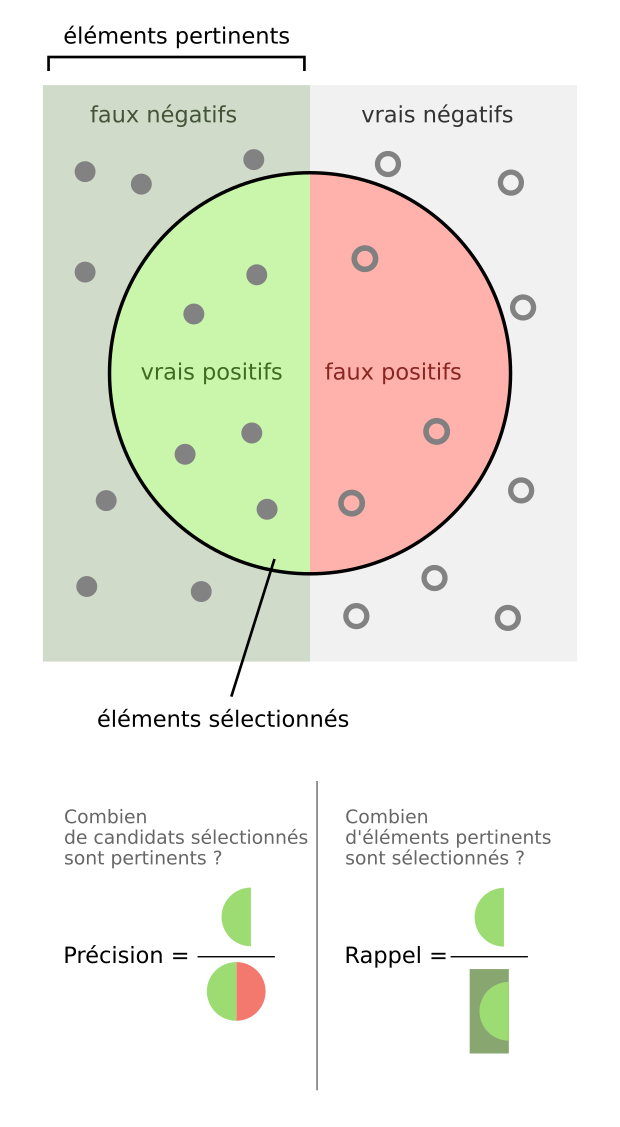
\includegraphics[width=0.3\textwidth]{./img/precision_recall.png}
    \caption{Précision et rappel (\textit{source:} \url{https://fr.wikipedia.org/wiki/Précision_et_rappel})}
    \label{precision_recall}
\end{figure}

\begin{figure}[h]
    \centering
    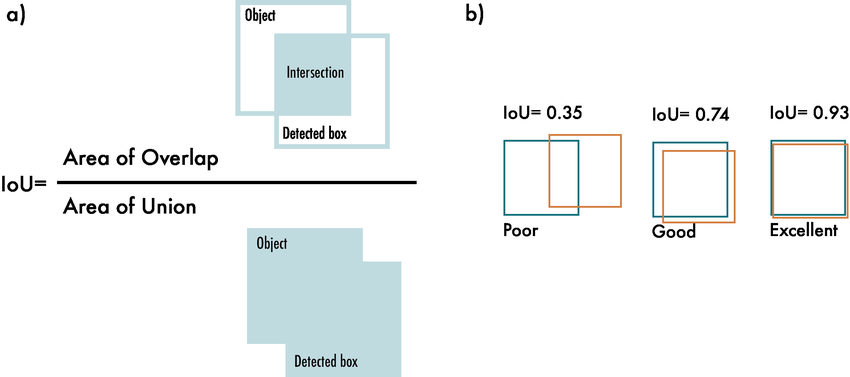
\includegraphics[width=0.5\textwidth]{./img/iou.png}
    \caption{Intersection over Union (\textit{source:}
    \cite{Terven_Cordova-Esparza_Ramirez-Pedraza_Chavez-Urbiola_2023})}
    \label{iou}
\end{figure}

\pagebreak

\chapter{Structure de YOLOX}


\begin{figure}[h]
    \centering
    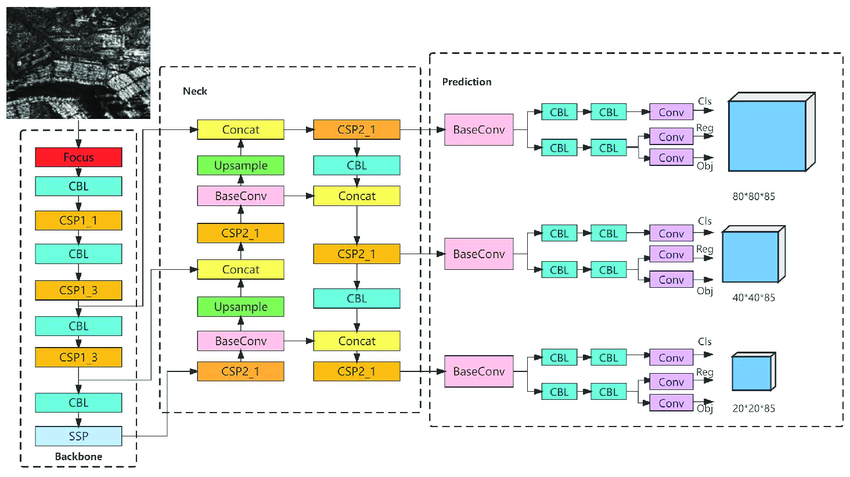
\includegraphics[width=0.5\textwidth]{./img/The-network-structure-of-YOLOX.png}
    \caption{Structure de YOLOX.}
    \label{yolox_structure}
\end{figure}


\begin{figure}[h]
    \centering
    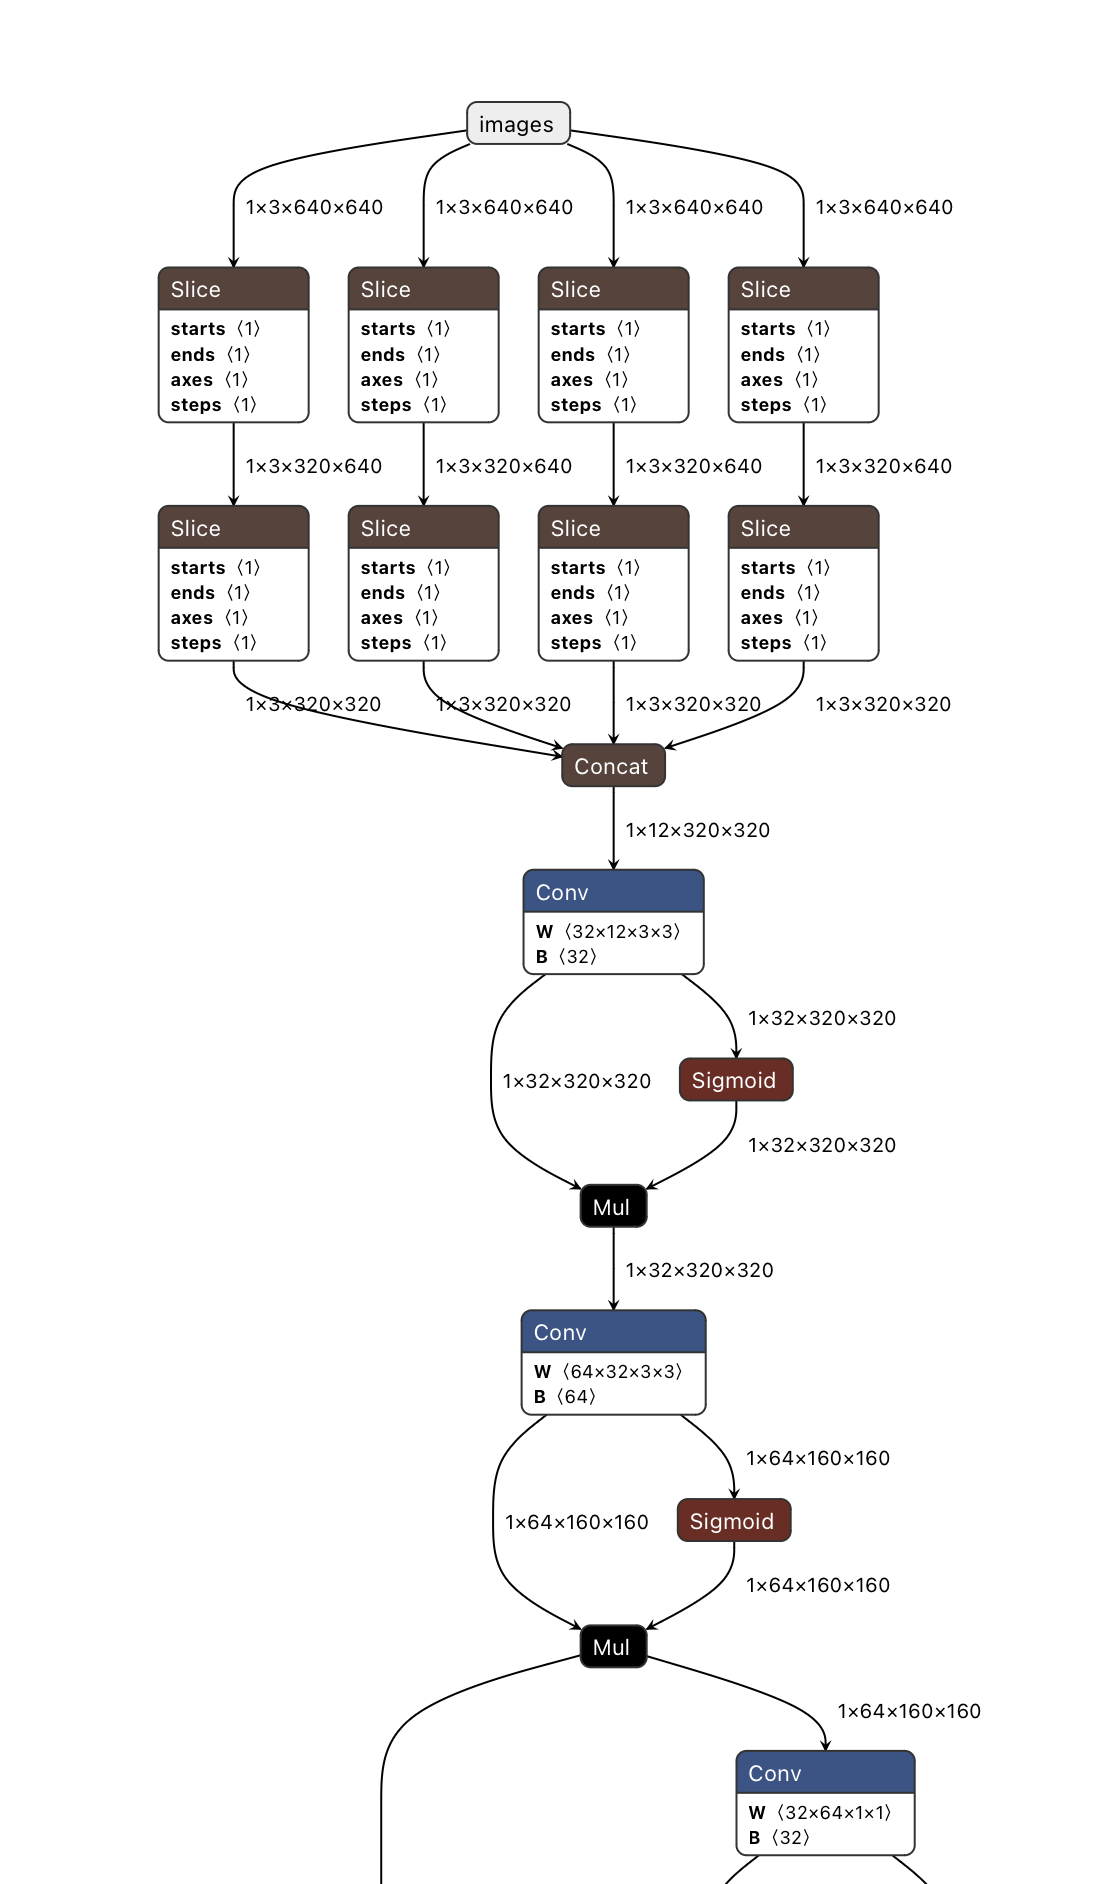
\includegraphics[width=0.5\textwidth]{./img/netron.png}
    \caption{Structure de YOLOX dans Netron.}
    \label{netron}
\end{figure}

\pagebreak

\chapter{Exemple de dictionnaire de conversion de labels (format json)}

\begin{verbatim}
{
    "vessel": "boat",
    "unknown": "boat",
    "commercial cargo-distant": "boat",
    "tug": "boat",
    "non-commercial small-human powered-blurry": "boat",
    "non-commercial medium-distant": "boat",
    "commercial cargo-blurry": "boat",
    "non-commercial sailing": "boat",
    "non-commercial small-backlit": "boat",
    "non-commercial small-dinghy": "boat",
    "non-commercial large-backlit": "boat",
    "commercial cargo": "boat",
    "other-backlit": "boat",
    "other-blurry": "boat",
    "non-commercial large": "boat",
    "non-commercial small-distant": "boat",
    "non-commercial sailing-blurry": "boat",
    "non-commercial small-dinghy-distant": "boat",
    [...]
    "non-commercial small-dinghy-blurry": "boat",
    "tug-blurry": "boat",
    "commercial small-blurry": "boat",
    "non-commercial small-blurry": "boat",
    "non-commercial large-distant": "boat",
    "commercial small": "boat",
    "commercial small-backlit": "boat",
    "other-tow-backlit": "boat",
    "non-commercial medium-backlit": "boat",
    "commercial large passenger-blurry": "boat",
    "non-commercial sailing-distant": "boat",
    "other-tow": "boat",
    "tug-backlit": "boat",
    "non-commercial medium-blurry": "boat",
    "tug-distant": "boat",
    "non-commercial large-blurry": "boat",
    "non-commercial sailing-backlit": "boat",
    "other": "boat",
    "non-commercial small-human powered-distant": "boat",
    "commercial large fishing-blurry": "boat",
    "unknown-distant": "boat"
}
\end{verbatim}
\label{ex_dictionnaire_conversion}

\pagebreak

\chapter{Définition des classes utilisées pour annoter les datasets}

\begin{itemize}
    \item \textbf{ferry}: Un navire utilisé pour le transport de personnes ou de marchandises.
    \item \textbf{warship}: Des navires militaires, des patrouilleurs ou d'autres navires utilisés par les forces militaires.
    \item \textbf{submarine} : Sous marin.
    \item \textbf{recreational}: Des petits bateaux légers fabriqués en matériau souple, des kayaks et des bateaux à pédale, ou des embarcations personnelles conçues pour le loisir ou la course.
    \item \textbf{luxury}: Des grand yachts luxueux conçus pour le plaisir.
    \item \textbf{sailboat} : Des petits voiliers utilisés pour le loisir ou la course.
    \item \textbf{service} : Des navires utilisés pour remorquer ou manœuvrer d'autres navires, les bateaux-pilotes ou les embarcations de sauvetage et de garde-côtes.
    \item \textbf{platform} : Des structures utilisées pour l'extraction pétrolière ou gazière.
    \item \textbf{fishing} : Un type de bateau utilisé pour la pêche ou le loisir.
    \item \textbf{bulker} : Des bateaux utilisés pour le transport de marchande en vrac (vraquiers).
    \item \textbf{cargo} : Des grands navires conçus pour transporter des marchandises dans des conteneurs standardisés.
    \item \textbf{cruise} : bateaux de croisière.
    \item \textbf{buoy} : bouées.
    \item \textbf{breakwater} : des jetées ou structure destinées à réduire l'impact des vagues.
    \item \textbf{lighthouse} : phares et structure de localisation.
\end{itemize}
\label{classes_annotations}

\pagebreak

\chapter{Interfaces}

\begin{landscape}
Interface de FiftyOne pour l'annotation de datasets : \\
    \begin{figure}[H]
        \centering
        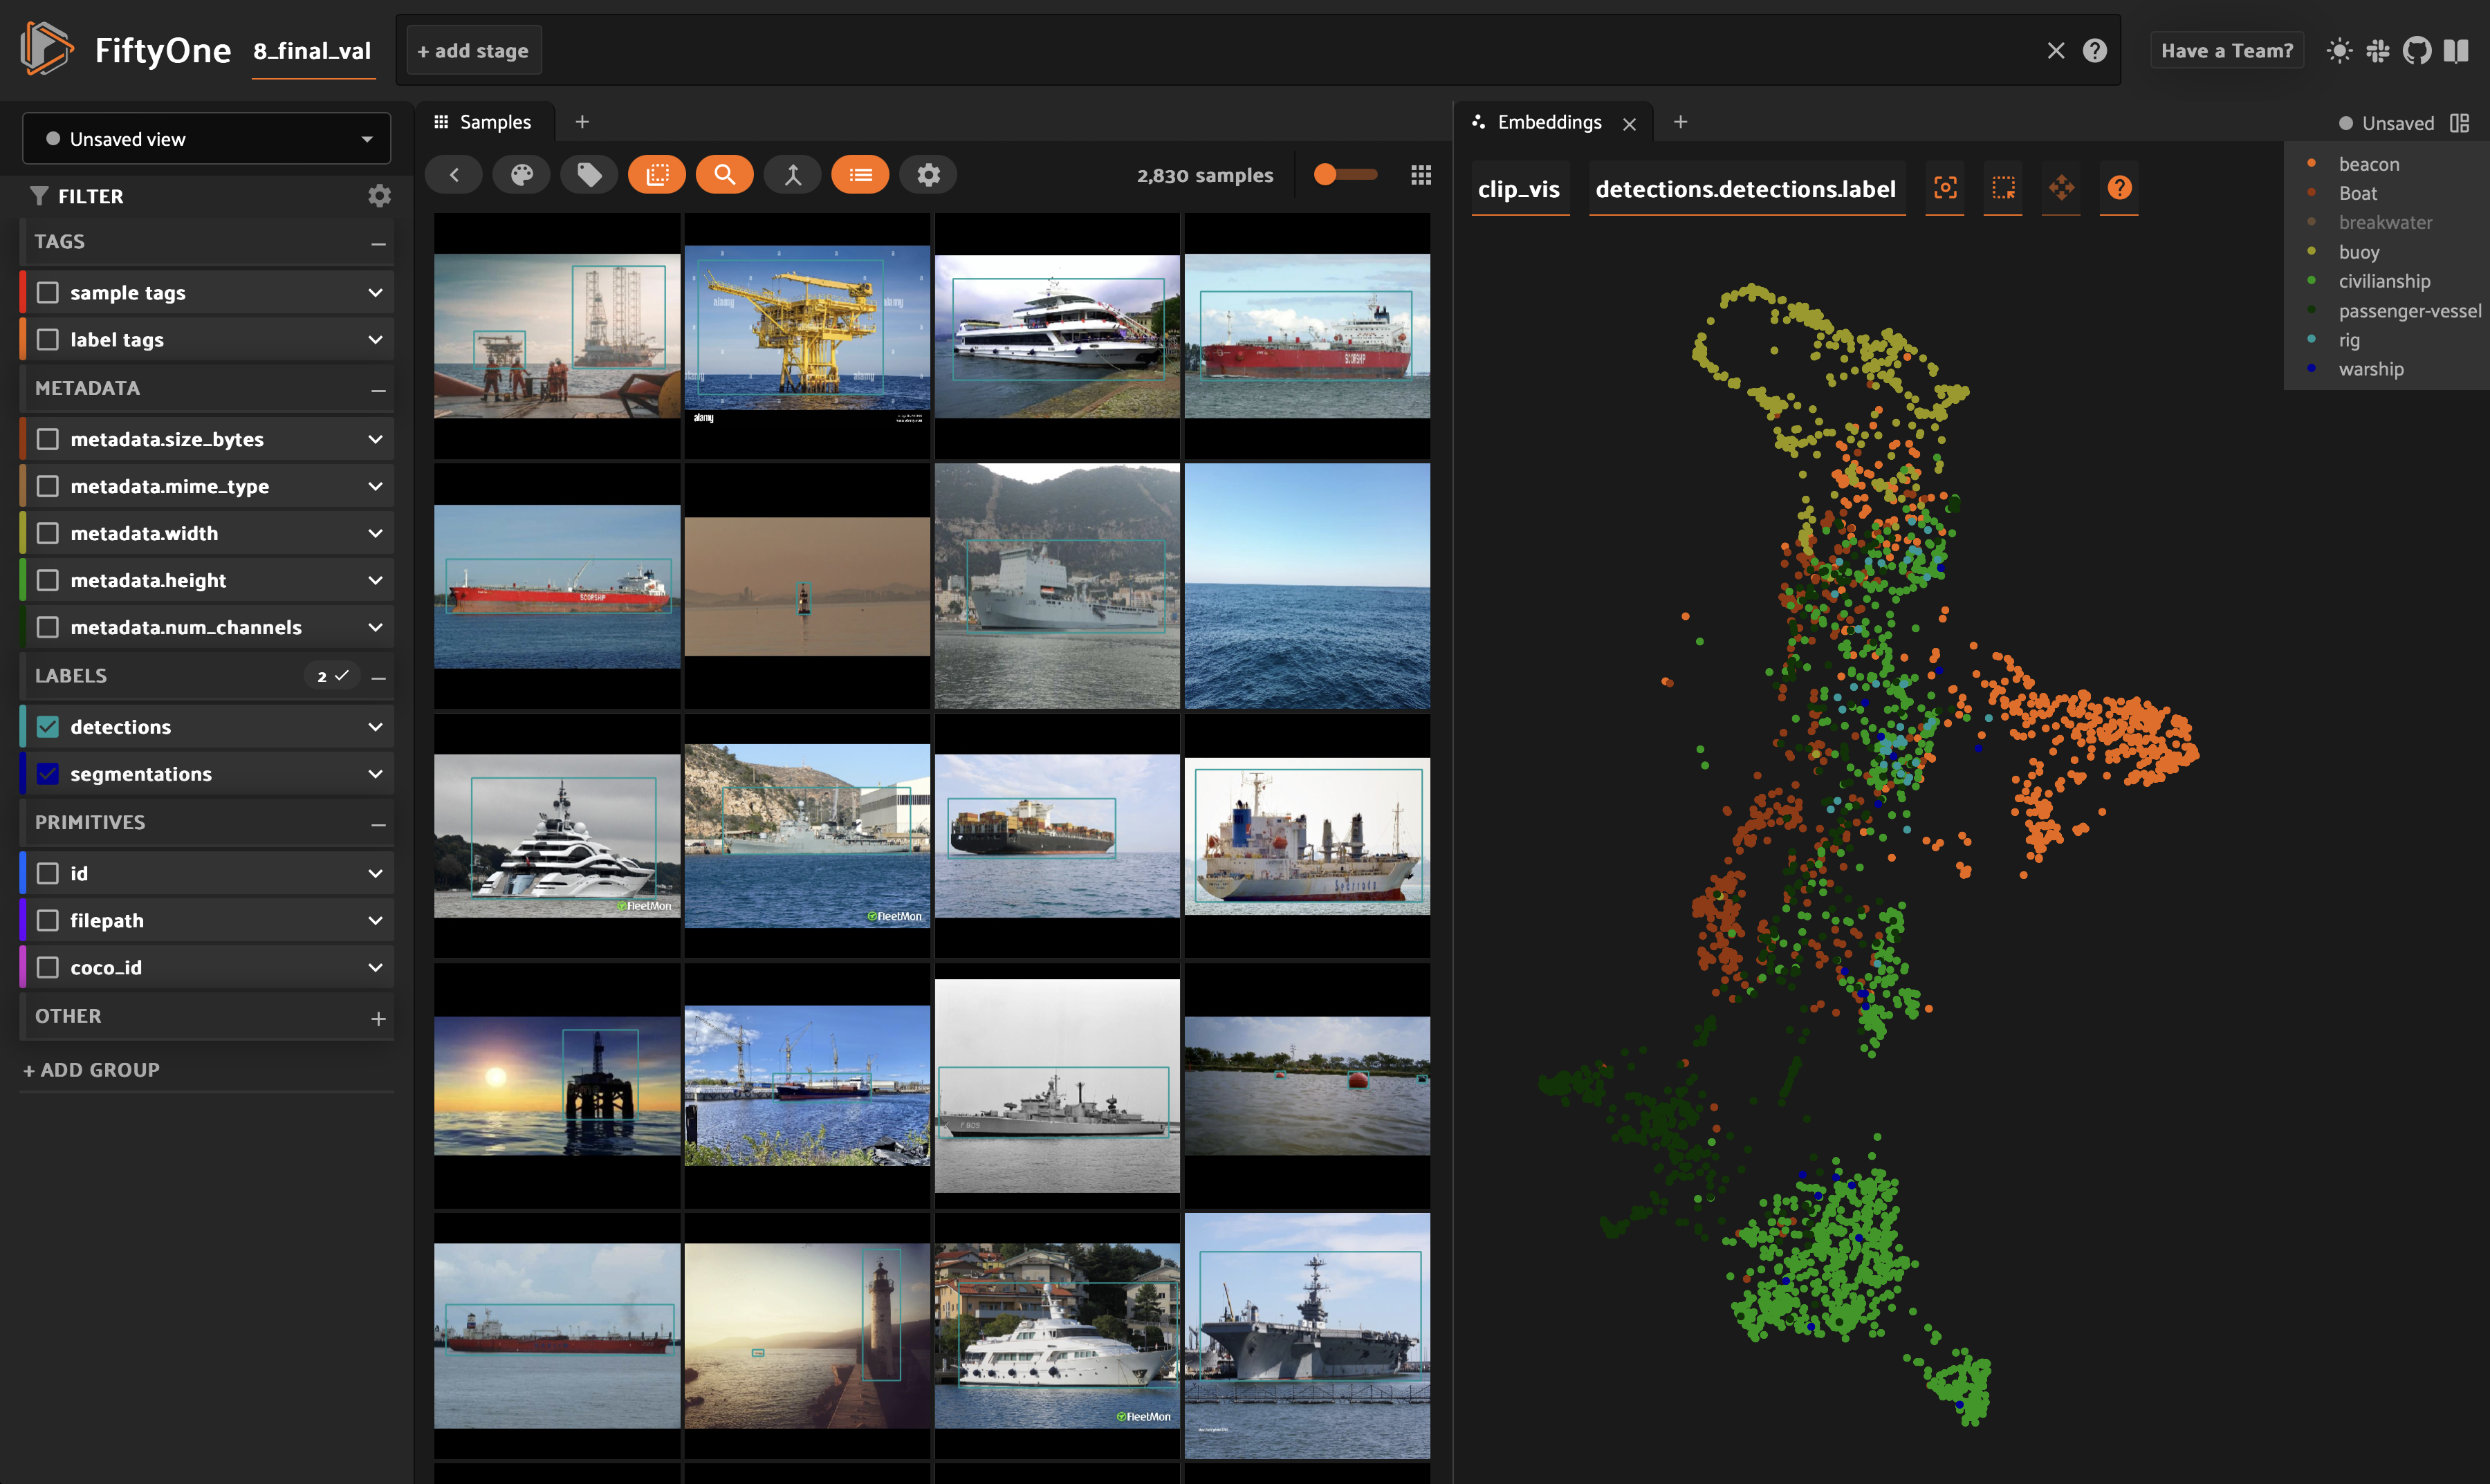
\includegraphics[width=1.4\textwidth]{clustering_interface.png}
        \caption{Interface pour l'annotation de datasets (\textit{carte de similarité à droite,
        une couleur par cluster K-Means})}
    \end{figure}\label{clustering_interface}
\end{landscape}

\pagebreak

\begin{landscape}
    DebuggerTool : \\
        \begin{figure}[H]
            \centering
            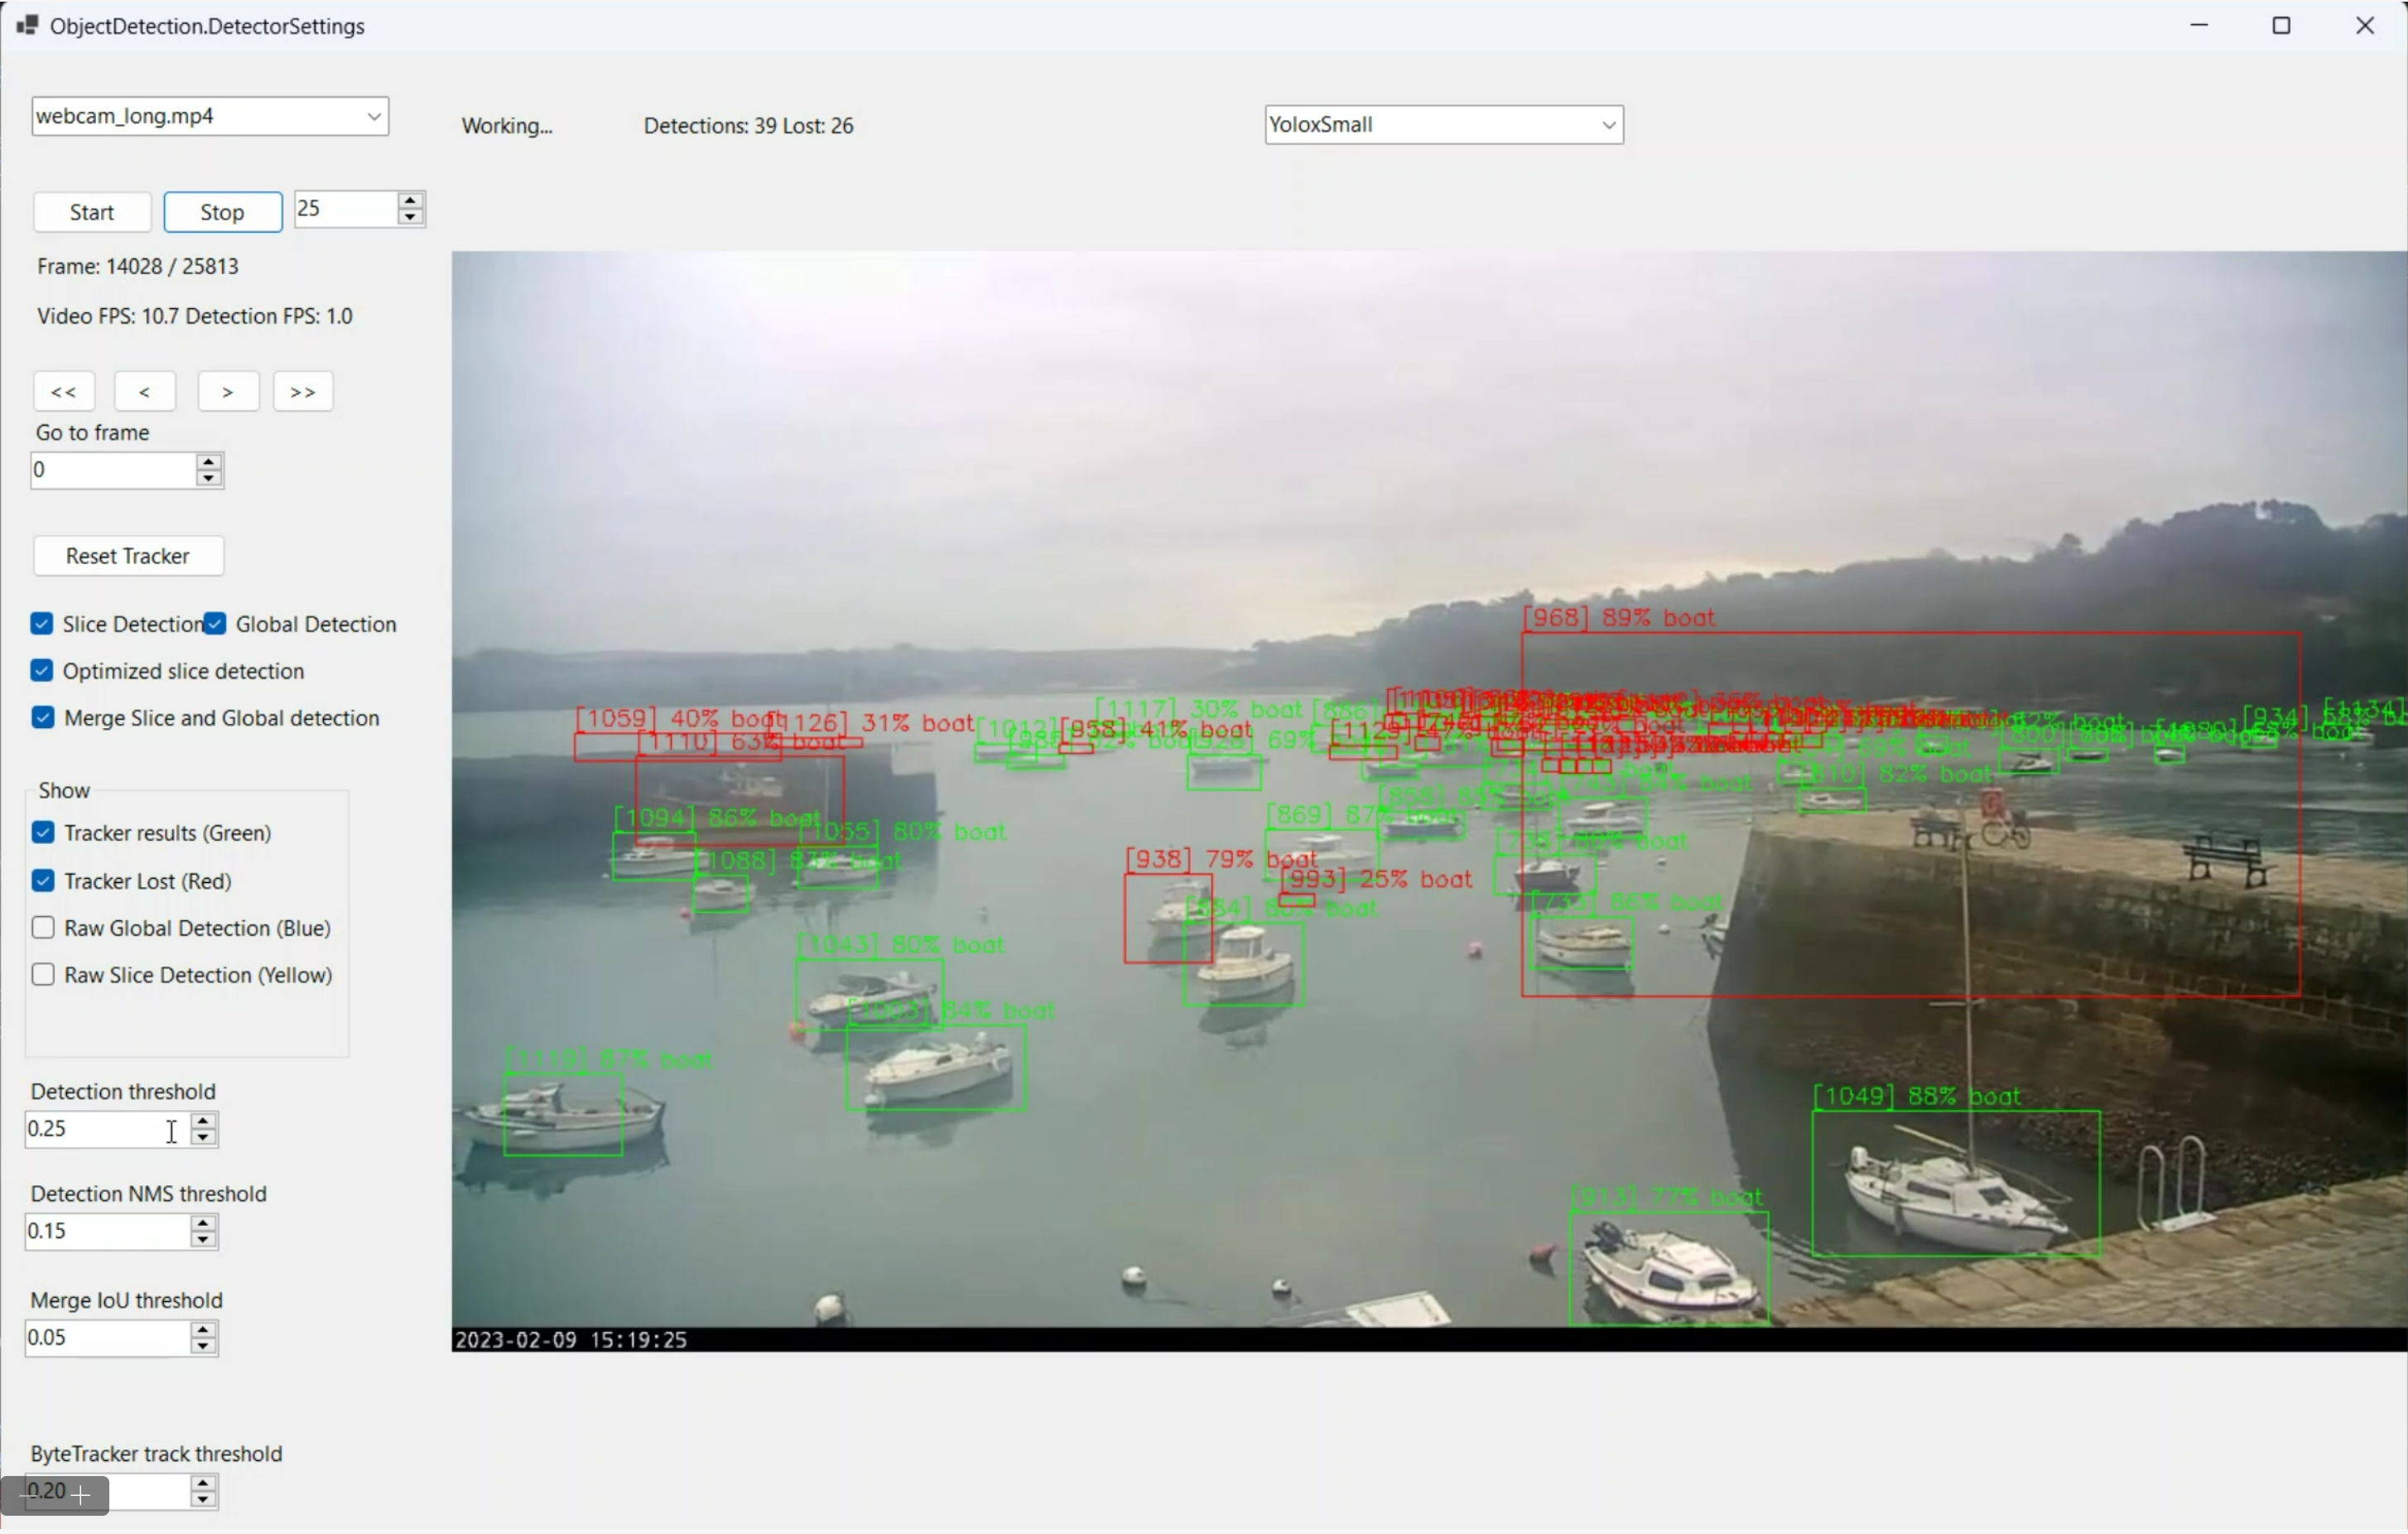
\includegraphics[width=1.4\textwidth]{debuggertool.png}
        \end{figure}\label{debuggertool}
    \end{landscape}
